\documentclass{classrep}
\usepackage[utf8]{inputenc}
\frenchspacing

\usepackage{graphicx}
\usepackage[usenames,dvipsnames]{color}
\usepackage[hidelinks]{hyperref}
\usepackage{lmodern}
\usepackage{placeins}
\usepackage{url}
\usepackage{amsmath, amssymb, mathtools}
\usepackage{listings}
\usepackage{fancyhdr, lastpage}
\usepackage{rotating}
\usepackage{makecell}
\usepackage{float}
\usepackage{multirow}

\pagestyle{fancyplain}
\fancyhf{}
\renewcommand{\headrulewidth}{0pt}
\cfoot{\thepage\ / \pageref*{LastPage}}

%--------------------------------------------------------------------------------------%
\studycycle{Informatyka stosowana, studia dzienne, II st.}
\coursesemester{I}

\coursename{Wprowadzenie do Data Science i metod uczenia maszynowego}
\courseyear{2020/2021}

\courseteacher{mgr inż. Rafał Woźniak}
\coursegroup{Wtorek, 13:15}

\author{%
    \studentinfo[239661@edu.p.lodz.pl]{Szymon Gruda}{239661}\\
    \studentinfo[239671@edu.p.lodz.pl]{Jan Karwowski}{239671}\\
    \studentinfo[239673@edu.p.lodz.pl]{Michał Kidawa}{239673}\\
    \studentinfo[239676@edu.p.lodz.pl]{Kamil Kowalewski}{239676}\\
}

\title{Zadanie 3.: Problem Set 3}

\begin{document}
    \maketitle
    \thispagestyle{fancyplain}

    \newpage
    \tableofcontents
    \newpage

    \section{Wprowadzenie}
    \label{intro} {

        \subsection{Opis zbiorów danych}
        \label{opis_zbiorow_intro} {

            \subsubsection{Zbiór Heart Disease UCI}
            \label{opis_zbiorow_intro_heart} {
                \begin{itemize}
                    \item \textbf{age} -- wiek w latach
                    \item \textbf{sex} -- płeć, gdzie 1 to mężczyzna a 0 to kobieta  
                    \item \textbf{cp (chest-pain-type)} -- rodzaj bólu w klatce piersiowej, przyjmuje wartość 0, 1, 2 lub 3  
                    \item  \textbf{trestbps (resting-blood-pressure)} -- ciśnienie krwi w czasie spoczynku (w mm/Hg przy przyjęciu do szpitala) 
                    \item \textbf{chol (serum-cholestoral)} -- cholesterol w surowicy w mg/dl  
                    \item \textbf{fbs (fasting-blood-sugar)} -- poziom cukru we krwi na czco, przyjmuje wartość 1 dla  poziomu większego niż 120 mg/dl, lub wartość 0 dla poziomu mniejszego
                    \item \textbf{restecg (resting-electrocardiographic)} -- wyniki eloktrokardiografu w spoczynku, przyjmuje wartość 0, 1 lub 2    stanie
                    \item \textbf{thalach (maximum-heart-rate)} -- najwyższe osiągnięte tętno   
                    \item \textbf{exang (exercise-induced-angina}) -- dławica wysiłkowa, przyjmuje wartość 1, jeżeli dławica występuje, w przeciwnym razie przyjmuje wartość 0
                    \item \textbf{oldpeak} -- Obniżenie odcinka ST, wywołane przez ćwiczenie, w stosunku do odpoczynku   
                    \item \textbf{slope (the-slope-of-the-peak-exercise)} -- nachylenie szczytowe odcinka ST podczas wysiłku, przyjmuje wartość 0, 1 lub 2  
                    \item \textbf{ca (number-of-major-vessels)} -- liczba głównych naczyń, przyjmuje wartość 0, 1, 2, 3 lub 4  
                    \item \textbf{thal} -- przyjmuje wartość 0, 1, 2 lub 3   
                    \item \textbf{target} -- przyjmuje wartość 0 lub 1 
                \end{itemize}
                }
                
                \subsubsection{Zbiór Gestures}
                \label{opis_zbiorow_intro_gestures} {
                    Zbiór posiada 65 kolumn w tym 8*8 pomiarów z sensorów. Dana osoba miała 
                   umieszczonych 8 czujników i każdy z nich zwracał 8 wartości co daje 64 kolumny 
                   oraz ostatnia 65 kolumnę czyli \textit{GESTURE\_CLASS}
                }

                \subsubsection{Zbiór Weather}
                \label{opis_zbiorow_intro_weather} {
                    \begin{itemize}
                        \item \textbf{Date} -- numer dnia roku wykonania pomiaru
                        \item \textbf{Location} -- miejsce pomiaru zamienione na liczbe
                        \item \textbf{MinTemp} -- minimalna tempeteratura
                        \item \textbf{MaxTemp} -- maksymalna tempeteratura
                        \item \textbf{Rainfall} -- opad deszczu w mm
                        \item \textbf{Evaporation} -- parowanie
                        \item \textbf{Sunshine} -- liczba godzin, w których swieci słońce
                        \item \textbf{WindGustDir} -- kierunek wiatru
                        \item \textbf{WindGustSpeed} -- siła wiatru
                        \item \textbf{WindDir9am} -- kierunek wiatru o godzinie 9 rano
                        \item \textbf{WindDir3pm} -- kierunek wiatru o godzinie 15
                        \item \textbf{WindSpeed9am} -- siła wiatru o godzinie 9 rano
                        \item \textbf{WindSpeed3pm} -- siła wiatru o godzinie 15
                        \item \textbf{Humidity9am} -- wilgotność o godzinie 9 rano
                        \item \textbf{Humidity3pm} -- wilgotność o godzinie 15
                        \item \textbf{Pressure9am} -- ciśnienie atmosferyczne o godzinie 9 rano
                        \item \textbf{Pressure3pm} -- ciśnienie atmosferyczne o godzinie 15
                        \item \textbf{Cloud9am} -- zachmurzenie o godzinie 9 rano
                        \item \textbf{Cloud3pm} -- zachmurzenie o godzinie 15
                        \item \textbf{Temp9am} -- temperatura o godzinie 9 rano
                        \item \textbf{Temp3pm} -- temperatura o godzinie 15
                        \item \textbf{RainToday} -- wartość logiczna - jeśli opady do godziny 9
                        rano były powyżej 1mm to wartość 1 jeśli nie to 0
                        \item \textbf{RainTomorrow} -- target variable 
                    \end{itemize}
                 }
        }

        \subsection{K-najbliższych sąsiadów}
        \label{knn_intro} {
            Zadanie klasyfikacji, polegające na przydzielaniu obiektów do wcześniej
            zdefiniowanych grup
            można rozwiązać na różne sposoby. Powstało wiele algorytmów
            klasyfikujących, a spośród nich
            jednym z najprostszych co do zasady działania jest algorytm
            k-NN (\emph{ang. k-nearest neighbors}).
            Klasyfikator ten nie wymaga procesu uczenia, zbiór uczący jest jedynie
            przechowywany w pamięci
            programu a przetwarzany jest dopiero podczas właściwej klasyfikacji.
            Działanie tego algorytmu polega
            na znajdowaniu najbliższych (zgodnie z pewną miarą) obiektów ze zbioru
            uczącego dla każdego elementu
            ze zbioru testowego. Następnie klasa przetwarzanego obiektu zostaje
            rozpoznana jako najczęstsza spośród
            znalezionych wcześniej "sąsiadów". Algorytm można więc przedstawić w
            następujących krokach:
            \begin{enumerate}
                \item Weź jeden element ze zbioru testowego
                \item Znajdź $k$ najbliższych elementów ze zbioru uczącego
                \item Wybierz klasę najczęściej występującą pośród znalezionych elementów
                \item Wybrana klasa jest klasą rozpoznawanego elementu ze zbioru testowego
            \end{enumerate}
        }

        \subsection{Naiwny klasyfikator Bayesa}
        \label{bayes_intro} {
        % wprowadznie teoretyczne
            Naiwny klasyfikator Bayesa wykorzystuje w procesie klasyfikacji twierdzenie Bayesa:
            $$ P(A \mid B) = \frac{P(B \mid A) \, P(A)}{P(B)} $$
            gdzie:
            \begin{itemize}
                \item $A$, $B$ -- zdarzenia
                \item $P(A \mid B)$ -- prawdopodobieństwo zdarzenia $A$, o ile zajdzie $B$
                \item $P(B \mid A)$ -- prawdopodobieństwo zdarzenia $B$, o ile zajdzie $A$
                \item $P(A)$ -- prawdopodobieństwo wystąpienia zdarzenia $A$
                \item $P(B)$ -- suma prawdopodobieństw wszystkich potencjalnych skutków zdarzenia: $P(B)=\sum P(B\mid A)P(B)$
            \end{itemize}

            Model naiwnego klasyfikatora Bayesa zakłada, że cecha danej próbki jest
            niepowiązana z pozostałymi cechami i wskazuje na prawdopodobieństwo
            przynależności do danej klasy.
            
            Przy tym klasyfikatorze jedynym dostępnym parametrem był podział na dane
            treningowe i testowe. Dokładność klasyfikacji sprawdzono dla każdego ze zbiorów danych w
            zależności od podziału na zbiór uczący i testowy.
        }

        \subsection{Maszyna wektorów nośnych}
        \label{svm_intro} {
            Maszyna wektorów nośnych - SVM (ang. Support Vector Machines) jako
            klasyfikator danych wykorzystuje przestrzeń decyzyjną, którą dzieli się
            budując granice separujące obiekty o różnej przynależności klasowej.
            Warunkiem jest to aby dzielone zbiory były liniowo separowalne, niestety
            jest rzadko spotykane -- tylko trywialne przykłady zbiorów charakteryzują
            się tą własnością. Na szczęście wykorzystanie funkcji jądrowych (ang.
            kernel functions) umożliwia przekształcenie każdego zbioru tak, aby
            charakteryzował się on liniową separalnością danych. W takim wypadku można
            poprowadzić nieskończenie wiele płaszczyzn dzielących klasy. Aby wybrać
            konkretną stosuję się metodę maksymalizacji marginesu -- dąży się do tego
            aby najbliższe dla hiperpłaszczyzny obiekty z danego obszaru były jak
            najbardziej od niej oddalone. Podstawowa implementacja maszyny wektorów
            nośnych uniemożliwia znalezienie się obiektu klasy A, po stronie
            hiperpłaszczyzny, na której znajdują się obiekty klasy B. Takie zachowanie
            powoduje pewne problemy, jak np. nadmierne dopasowanie modelu. Rozwiązaniem
            tego problemu jest nadanie odpowiedniej wartości parametrowi \emph{C},
            który jest odpowiedzialny za tolerancję zjawiska, w którym niektóre obiekty
            znajdują się po nieprawidłowej stronie hiperpłaszczyzny. Natomiast wartość
            parametru gamma (dostępnego tylko dla niektórych funkcji jądra) określa
            promień pojedynczego punktu, w jakiego odległości musi się znaleźć inny
            punkt, aby zostały one zgrupowane razem.
        }

        \subsection{Drzewa decyzyjne i lasy losowe}
        \label{drzewa_decyzyjne_intro} {
            Drzewa decyzyjne to bardzo prosty i jednocześnie skuteczny klasyfikator. Na
            podstawie zbioru danych uczących buduje się drzewo, gdzie każdy węzeł
            pośredni zawiera pewien warunek (cechę i jej wartość graniczną), według
            którego dzieli się zbiór uczący na dwie części (w przypadku biblioteki
            scikit-learn są to drzewa binarne). Następnie każdą taką część znowu dzieli
            się na kolejne wybierając kolejny warunek. Na każdym etapie podziały robi
            się w ten sposób, aby powstałe podzbiory zbioru uczącego były według pewnej
            miary jak najmniej zanieczyszczone, czyli aby podziały były na każdym
            etapie jak najlepsze. Węzły końcowe (liście) oznaczają konkretne klasy.
            Drzewo takie można budować aż do osiągnięcia idealnie czystych podzbiorów,
            co w najgorszym przypadku może oznaczać jeden liść na jeden przykład
            uczący, co z kolei wiąże się ze skrajnym przetrenowaniem modelu. Z tego
            powodu w przypadku uczenia drzew decyzyjnych zawsze wprowadza się parametry
            regularyzacyjne, takie jak maksymalna wysokość drzewa czy minimalna liczba
            przykładów uczących w liściu. Tak zbudowane drzewo decyzyjne można
            wykorzystać do rozpoznawania klasy nieznanego przykładu, poprzez
            "przejście" od korzenia drzewa aż do któregoś liścia, zgodnie z wartościami
            cech danego przykładu i warunkami w węzłach pośrednich.

            Las losowy jest niczym innym jak zespołem drzew, gdzie każde może być
            wyuczone wykorzystując jedynie pewien podzbiór zbioru uczącego. W ten
            sposób powstaje pewna liczba klasyfikatorów, każdy trochę inny,
            popełniający inne błędy. W celu znalezienia klasy zadanego przykładu
            wybiera się tę, która jest najczęściej wskazywana przez wszystkie drzewa w
            lesie. W ten sposób uzyskuje się znacznie bardziej uniwersalny i model,
            lepiej generalizujący i lepiej radzący sobie w przypadku zbiorów z dużą
            wariancją.
        }
    }
    \newpage
    
    \section{Wyniki}
    \label{results} {

        \subsection{K-najbliższych sąsiadów}
        \label{knn_results} {

            \subsubsection{Metryka Euklidesowa}
            \label{knn_results_eucl} {

                \begin{table}[!htbp]
                    \begin{minipage}{.35\textwidth}
                        \centering
                        \begin{tabular}{|c|c|}
                            \hline
                            K & Accuracy \\ \hline
                            1 & 0.6264 \\ \hline
                            2 & 0.5824 \\ \hline
                            3 & 0.6703 \\ \hline
                            4 & 0.6703 \\ \hline
                            5 & 0.6593 \\ \hline
                            6 & 0.6374 \\ \hline
                            7 & 0.6813 \\ \hline
                            8 & 0.7143 \\ \hline
                            9 & 0.7143 \\ \hline
                            10 & 0.7253 \\ \hline
                            11 & 0.7033 \\ \hline
                            12 & 0.6703 \\ \hline
                            13 & 0.6593 \\ \hline
                            14 & 0.6374 \\ \hline
                            15 & 0.6484 \\ \hline
                            16 & 0.6484 \\ \hline
                            17 & 0.6703 \\ \hline
                            18 & 0.6813 \\ \hline
                            19 & 0.6703 \\ \hline
                            20 & 0.6593 \\ \hline
                            21 & 0.6923 \\ \hline
                            22 & 0.6813 \\ \hline
                            23 & 0.7033 \\ \hline
                            24 & 0.6593 \\ \hline
                            25 & 0.6593 \\ \hline
                            26 & 0.6593 \\ \hline
                            27 & 0.6813 \\ \hline
                            28 & 0.6813 \\ \hline
                            29 & 0.6923 \\ \hline
                        \end{tabular}
                        \caption
                        [knn table heart eucl]{Zbiór heart disease}
                        \label{knn_table_heart_eucl}
                    \end{minipage}
                    \hfill
                    \begin{minipage}{.3\textwidth}
                        \centering
                        \begin{tabular}{|c|c|}
                            \hline
                            K & Accuracy \\ \hline
                            1 & 0.6644 \\ \hline
                            2 & 0.6655 \\ \hline
                            3 & 0.6835 \\ \hline
                            4 & 0.6855 \\ \hline
                            5 & 0.6781 \\ \hline
                            6 & 0.6812 \\ \hline
                            7 & 0.6812 \\ \hline
                            8 & 0.6838 \\ \hline
                            9 & 0.6821 \\ \hline
                            10 & 0.6807 \\ \hline
                            11 & 0.6801 \\ \hline
                            12 & 0.6738 \\ \hline
                            13 & 0.6801 \\ \hline
                            14 & 0.6747 \\ \hline
                            15 & 0.6741 \\ \hline
                            16 & 0.6712 \\ \hline
                            17 & 0.6712 \\ \hline
                            18 & 0.6701 \\ \hline
                            19 & 0.6698 \\ \hline
                            20 & 0.6701 \\ \hline
                            21 & 0.6624 \\ \hline
                            22 & 0.6621 \\ \hline
                            23 & 0.6572 \\ \hline
                            24 & 0.657 \\ \hline
                            25 & 0.6587 \\ \hline
                            26 & 0.6558 \\ \hline
                            27 & 0.6592 \\ \hline
                            28 & 0.6584 \\ \hline
                            29 & 0.6587 \\ \hline
                        \end{tabular}
                        \caption
                        [knn table gestures eucl]{Zbiór gestures}
                        \label{knn_table_gestures_eucl}
                    \end{minipage}
                    \hfill
                    \begin{minipage}{.3\textwidth}
                        \centering
                        \begin{tabular}{|c|c|}
                            \hline
                            K & Accuracy \\ \hline
                            1 & 0.8117 \\ \hline
                            2 & 0.8284 \\ \hline
                            3 & 0.8348 \\ \hline
                            4 & 0.8394 \\ \hline
                            5 & 0.8434 \\ \hline
                            6 & 0.8447 \\ \hline
                            7 & 0.8472 \\ \hline
                            8 & 0.8457 \\ \hline
                            9 & 0.849 \\ \hline
                            10 & 0.847 \\ \hline
                            11 & 0.8505 \\ \hline
                            12 & 0.8503 \\ \hline
                            13 & 0.8516 \\ \hline
                            14 & 0.8508 \\ \hline
                            15 & 0.8525 \\ \hline
                            16 & 0.85 \\ \hline
                            17 & 0.8514 \\ \hline
                            18 & 0.8499 \\ \hline
                            19 & 0.8509 \\ \hline
                            20 & 0.8496 \\ \hline
                            21 & 0.8509 \\ \hline
                            22 & 0.8495 \\ \hline
                            23 & 0.8514 \\ \hline
                            24 & 0.8502 \\ \hline
                            25 & 0.8526 \\ \hline
                            26 & 0.8503 \\ \hline
                            27 & 0.8524 \\ \hline
                            28 & 0.8511 \\ \hline
                            29 & 0.8524 \\ \hline
                        \end{tabular}
                        \caption
                        [knn table weather eucl]{Zbiór weather AUS}
                        \label{knn_table_weather_eucl}
                    \end{minipage}
                \end{table}
                \FloatBarrier

                \begin{figure}[!htbp]
                    \centering
                    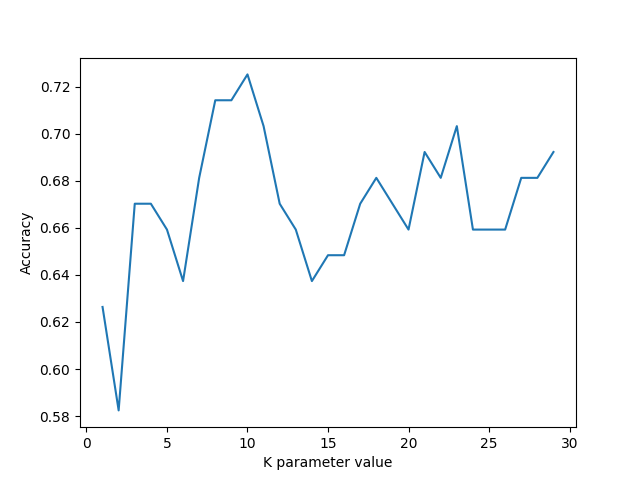
\includegraphics
                    [width=\textwidth,keepaspectratio]
                    {img/knn_chart_heart_eucl-193604.png}
                    \caption
                    [knn chart heart eucl 193604]{Zbiór heart disease}
                    \label{knn_chart_heart_eucl-193604}
                \end{figure}

                \begin{figure}[!htbp]
                    \centering
                    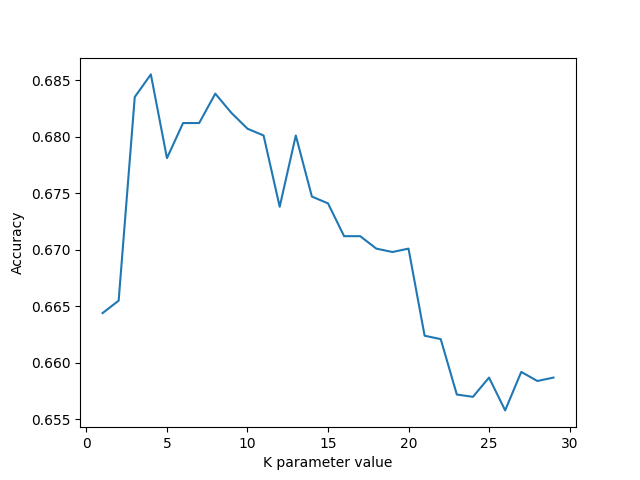
\includegraphics
                    [width=\textwidth,keepaspectratio]
                    {img/knn_chart_gestures_eucl-193709.png}
                    \caption
                    [knn chart gestures eucl 193709]{Zbiór gestures}
                    \label{knn_chart_gestures_eucl-193709}
                \end{figure}

                \begin{figure}[!htbp]
                    \centering
                    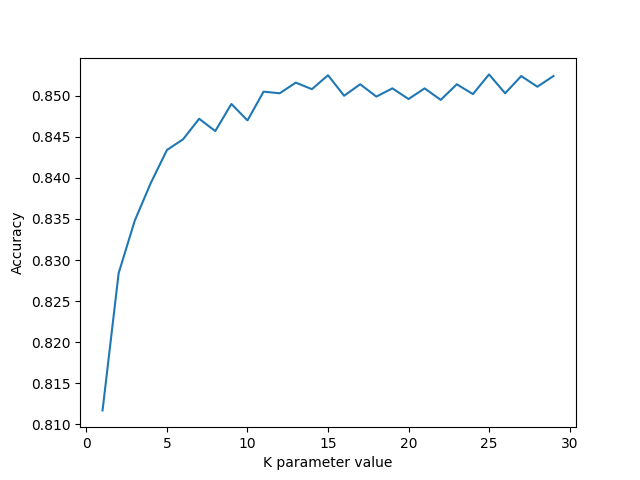
\includegraphics
                    [width=\textwidth,keepaspectratio]
                    {img/knn_chart_weather_eucl-195550.png}
                    \caption
                    [knn chart weather eucl 195550]{Zbiór weather AUS}
                    \label{knn_chart_weather_eucl-195550}
                \end{figure}
                \FloatBarrier
            }

            \subsubsection{Metryka Manhattan}
            \label{knn_results_manh} {

                \begin{table}[!htbp]
                    \begin{minipage}{.35\textwidth}
                        \centering
                        \begin{tabular}{|c|c|}
                            \hline
                            K & Accuracy \\ \hline
                            1 & 0.6044 \\ \hline
                            2 & 0.6703 \\ \hline
                            3 & 0.7253 \\ \hline
                            4 & 0.7363 \\ \hline
                            5 & 0.7363 \\ \hline
                            6 & 0.7253 \\ \hline
                            7 & 0.7363 \\ \hline
                            8 & 0.7143 \\ \hline
                            9 & 0.6923 \\ \hline
                            10 & 0.7033 \\ \hline
                            11 & 0.7033 \\ \hline
                            12 & 0.6923 \\ \hline
                            13 & 0.7033 \\ \hline
                            14 & 0.7033 \\ \hline
                            15 & 0.7253 \\ \hline
                            16 & 0.7033 \\ \hline
                            17 & 0.6813 \\ \hline
                            18 & 0.6813 \\ \hline
                            19 & 0.7143 \\ \hline
                            20 & 0.6923 \\ \hline
                            21 & 0.7143 \\ \hline
                            22 & 0.7253 \\ \hline
                            23 & 0.7033 \\ \hline
                            24 & 0.6923 \\ \hline
                            25 & 0.6813 \\ \hline
                            26 & 0.6813 \\ \hline
                            27 & 0.6813 \\ \hline
                            28 & 0.6593 \\ \hline
                            29 & 0.6923 \\ \hline
                        \end{tabular}
                        \caption
                        [knn table heart manh]{Zbiór heart disease}
                        \label{knn_table_heart_manh}
                    \end{minipage}
                    \hfill
                    \begin{minipage}{.3\textwidth}
                        \centering
                        \begin{tabular}{|c|c|}
                            \hline
                            K & Accuracy \\ \hline
                            1 & 0.6555 \\ \hline
                            2 & 0.6504 \\ \hline
                            3 & 0.6667 \\ \hline
                            4 & 0.6564 \\ \hline
                            5 & 0.6764 \\ \hline
                            6 & 0.6672 \\ \hline
                            7 & 0.6741 \\ \hline
                            8 & 0.6675 \\ \hline
                            9 & 0.6692 \\ \hline
                            10 & 0.6672 \\ \hline
                            11 & 0.6729 \\ \hline
                            12 & 0.663 \\ \hline
                            13 & 0.6627 \\ \hline
                            14 & 0.6604 \\ \hline
                            15 & 0.6604 \\ \hline
                            16 & 0.6587 \\ \hline
                            17 & 0.6564 \\ \hline
                            18 & 0.6564 \\ \hline
                            19 & 0.6558 \\ \hline
                            20 & 0.6515 \\ \hline
                            21 & 0.6507 \\ \hline
                            22 & 0.6484 \\ \hline
                            23 & 0.6478 \\ \hline
                            24 & 0.6473 \\ \hline
                            25 & 0.6484 \\ \hline
                            26 & 0.6404 \\ \hline
                            27 & 0.6424 \\ \hline
                            28 & 0.6396 \\ \hline
                            29 & 0.6418 \\ \hline
                        \end{tabular}
                        \caption
                        [knn table gestures manh]{Zbiór gestures}
                        \label{knn_table_gestures_manh}
                    \end{minipage}
                    \hfill
                    \begin{minipage}{.3\textwidth}
                        \centering
                        \begin{tabular}{|c|c|}
                            \hline
                            K & Accuracy \\ \hline
                            1 & 0.8224 \\ \hline
                            2 & 0.8351 \\ \hline
                            3 & 0.8424 \\ \hline
                            4 & 0.8421 \\ \hline
                            5 & 0.847 \\ \hline
                            6 & 0.8446 \\ \hline
                            7 & 0.8516 \\ \hline
                            8 & 0.8498 \\ \hline
                            9 & 0.8535 \\ \hline
                            10 & 0.8505 \\ \hline
                            11 & 0.8532 \\ \hline
                            12 & 0.8518 \\ \hline
                            13 & 0.854 \\ \hline
                            14 & 0.8516 \\ \hline
                            15 & 0.8535 \\ \hline
                            16 & 0.8522 \\ \hline
                            17 & 0.8546 \\ \hline
                            18 & 0.8522 \\ \hline
                            19 & 0.8542 \\ \hline
                            20 & 0.8528 \\ \hline
                            21 & 0.8545 \\ \hline
                            22 & 0.8541 \\ \hline
                            23 & 0.855 \\ \hline
                            24 & 0.8537 \\ \hline
                            25 & 0.8542 \\ \hline
                            26 & 0.8528 \\ \hline
                            27 & 0.854 \\ \hline
                            28 & 0.8527 \\ \hline
                            29 & 0.8534 \\ \hline
                        \end{tabular}
                        \caption
                        [knn table weather manh]{Zbiór weather AUS}
                        \label{knn_table_weather_manh}
                    \end{minipage}
                \end{table}
                \FloatBarrier

                \begin{figure}[!htbp]
                    \centering
                    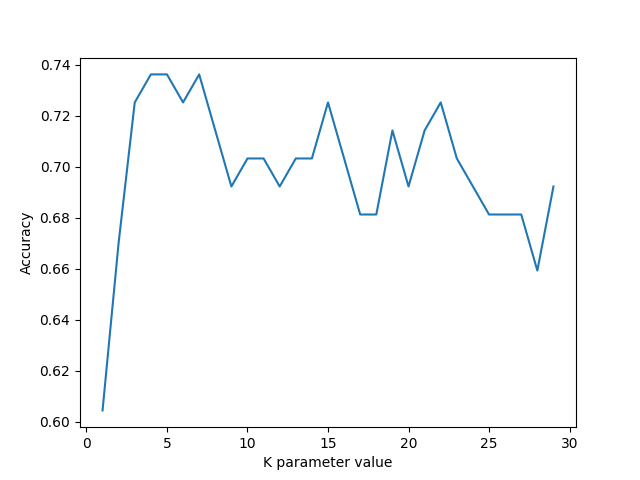
\includegraphics
                    [width=\textwidth,keepaspectratio]
                    {img/knn_chart_heart_manh-193605.png}
                    \caption
                    [knn chart heart manh 193605]{Zbiór heart disease}
                    \label{knn_chart_heart_manh-193605}
                \end{figure}

                \begin{figure}[!htbp]
                    \centering
                    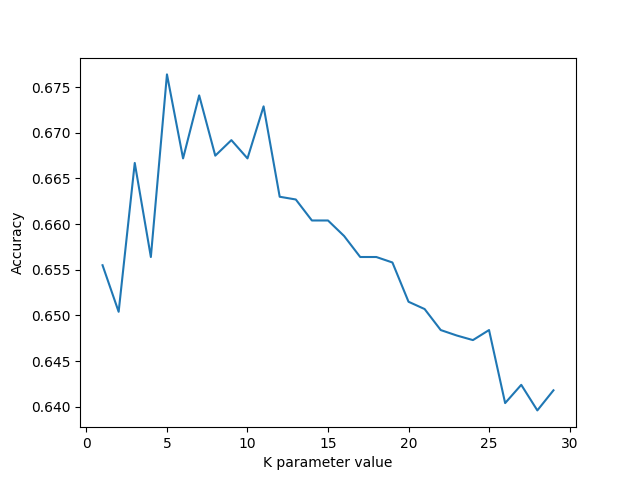
\includegraphics
                    [width=\textwidth,keepaspectratio]
                    {img/knn_chart_gestures_manh-193850.png}
                    \caption
                    [knn chart gestures manh 193850]{Zbiór gestures}
                    \label{knn_chart_gestures_manh-193850}
                \end{figure}

                \begin{figure}[!htbp]
                    \centering
                    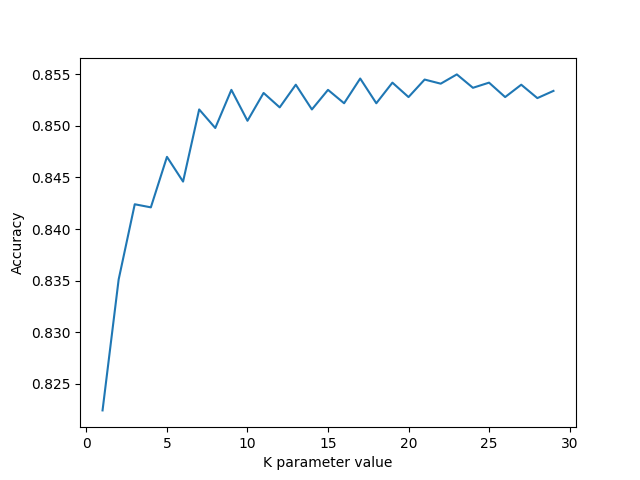
\includegraphics
                    [width=\textwidth,keepaspectratio]
                    {img/knn_chart_weather_manh-201711.png}
                    \caption
                    [knn chart weather manh 201711]{Zbiór weather AUS}
                    \label{knn_chart_weather_manh-201711}
                \end{figure}
                \FloatBarrier
            }
        }

        \subsection{Naiwny klasyfikator Bayesa}
        W przypadku eksperymentów wykorzystujących naiwny klasyfikator Bayesa jako
        parametr został przyjęty podział na dane uczące i testowe.
        
        \label{bayes_results} {
            \begin{table}[H]
                \centering
                \begin{tabular}{|c|c|c|c|}
                \hline
                \multirow{2}{*}{\textbf{\begin{tabular}[c]{@{}c@{}}\% danych\\ testowych\end{tabular}}} & \multicolumn{3}{c|}{\textbf{Zbiór danych}} \\ \cline{2-4} 
                        & \textbf{heart diseases}      & \textbf{gestures}     & \textbf{weather}     \\ \hline
                30 \%   & 0.8132           & 0.8779          & 0.8004          \\ \hline
                35 \%   & 0.8037           & 0.8826          & 0.7996          \\ \hline
                40 \%   & 0.8033           & 0.8859          & 0.8011          \\ \hline
                45 \%   & 0.7737           & 0.883          & 0.7991          \\ \hline
                50 \%   & 0.7961           & 0.8853          & 0.8002          \\ \hline
                55 \%   & 0.7784           & 0.8804          & 0.802         \\ \hline
                60 \%   &  0.7747           & 0.8804          & 0.8029         \\ \hline
                65 \%   &  0.7543           & 0.8803          & 0.8032         \\ \hline
                70 \%   &  0.7793           & 0.8802          & 0.8067         \\ \hline
                75 \%   &  0.7851           & 0.8842          & 0.8063         \\ \hline
                80 \%   &  0.786           & 0.884          & 0.8048         \\ \hline
                85 \%   &  0.7907           & 0.8816          & 0.8064         \\ \hline
                90 \%   &  0.7033           & 0.8826          & 0.8048         \\ \hline
                \end{tabular}
                \caption{Porównanie dokładności dla różnych zbiorów, dla naiwnego klasyfikatora Bayesa}
                \label{tab:bayes}
            \end{table}
        }

        \subsection{Maszyna wektorów nośnych}
        \label{svm_results} {
            W eksperymentach badających dokładność klasyfikatora opartego o maszynę
            wektorów nośnych sprawdzanie było zachowanie klasyfikatora (dokładność
            klasyfikacji) dla trzech różnych funkcji jądra:
            \begin{enumerate}
                \item wielomianowej - w skrócie poly
                \item radialnej funkcji bazowej (ang. radial basis function) - w
                \item skrócie RBF
                \item sigmoidalnej - w skrócie sigmoid
            \end{enumerate}
            Dla każdej funkcji zmieniano wartości parametru C, lub gamma.
        %HEARTH
            \begin{table}[!htbp]
                \begin{minipage}{.35\textwidth}
                    \centering
                    \begin{tabular}{|c|c|}
                        \hline
                        C & Accuracy \\ \hline
                        0.1 & 0.5275 \\ \hline
                        0.2 & 0.6264 \\ \hline
                        0.3 & 0.6484 \\ \hline
                        0.4 & 0.6813 \\ \hline
                        0.5 & 0.6813 \\ \hline
                        0.6 & 0.6703 \\ \hline
                        0.7 & 0.6813 \\ \hline
                        0.8 & 0.6813 \\ \hline
                        0.9 & 0.6923 \\ \hline
                        1.0 & 0.6923 \\ \hline
                        1.1 & 0.6923 \\ \hline
                        1.2 & 0.6923 \\ \hline
                        1.3 & 0.7033 \\ \hline
                        1.4 & 0.7143 \\ \hline
                        1.5 & 0.7143 \\ \hline
                        1.6 & 0.7253 \\ \hline
                        1.7 & 0.7253 \\ \hline
                        1.8 & 0.7253 \\ \hline
                        1.9 & 0.7253 \\ \hline
                        2.0 & 0.7253 \\ \hline
                    \end{tabular}
                    \caption
                    [svm table c heart poly]{Zbiór heart funkcja - wielomian}
                    \label{svm_table_c_heart_poly}
                \end{minipage}
                \hfill
                \begin{minipage}{.3\textwidth}
                    \centering
                    \begin{tabular}{|c|c|}
                        \hline
                        C & Accuracy \\ \hline
                        0.1 & 0.5275 \\ \hline
                        0.2 & 0.5275 \\ \hline
                        0.3 & 0.5275 \\ \hline
                        0.4 & 0.5714 \\ \hline
                        0.5 & 0.6044 \\ \hline
                        0.6 & 0.6154 \\ \hline
                        0.7 & 0.6593 \\ \hline
                        0.8 & 0.6593 \\ \hline
                        0.9 & 0.6484 \\ \hline
                        1.0 & 0.6593 \\ \hline
                        1.1 & 0.6593 \\ \hline
                        1.2 & 0.6813 \\ \hline
                        1.3 & 0.6813 \\ \hline
                        1.4 & 0.6813 \\ \hline
                        1.5 & 0.6813 \\ \hline
                        1.6 & 0.6813 \\ \hline
                        1.7 & 0.6923 \\ \hline
                        1.8 & 0.6923 \\ \hline
                        1.9 & 0.6923 \\ \hline
                        2.0 & 0.6813 \\ \hline
                    \end{tabular}
                    \caption
                    [svm table c heart rbf]{Zbiór heart funkcja - RBF}
                    \label{svm_table_c_heart_rbf}
                \end{minipage}
                \hfill
                \begin{minipage}{.3\textwidth}
                    \centering
                    \begin{tabular}{|c|c|}
                        \hline
                        C & Accuracy \\ \hline
                        0.1 & 0.5275 \\ \hline
                        0.2 & 0.5275 \\ \hline
                        0.3 & 0.5275 \\ \hline
                        0.4 & 0.5275 \\ \hline
                        0.5 & 0.5275 \\ \hline
                        0.6 & 0.5275 \\ \hline
                        0.7 & 0.5275 \\ \hline
                        0.8 & 0.5275 \\ \hline
                        0.9 & 0.5275 \\ \hline
                        1.0 & 0.5275 \\ \hline
                        1.1 & 0.5275 \\ \hline
                        1.2 & 0.5275 \\ \hline
                        1.3 & 0.5275 \\ \hline
                        1.4 & 0.5275 \\ \hline
                        1.5 & 0.5385 \\ \hline
                        1.6 & 0.5604 \\ \hline
                        1.7 & 0.5495 \\ \hline
                        1.8 & 0.5824 \\ \hline
                        1.9 & 0.6044 \\ \hline
                        2.0 & 0.6374 \\ \hline
                    \end{tabular}
                    \caption
                    [svm table c heart sigmoid]{Zbiór weather funkcja - Sigmoidalna}
                    \label{svm_table_c_heart_sigmoid}
                \end{minipage}
            \end{table}
            \FloatBarrier
            \begin{table}[!htbp]
                \begin{minipage}{.35\textwidth}
                    \centering
                    \begin{tabular}{|c|c|}
                        \hline
                        Gamma & Accuracy \\ \hline
                        1e-20 & 0.5275 \\ \hline
                        1e-19 & 0.5275 \\ \hline
                        1e-18 & 0.5275 \\ \hline
                        1e-17 & 0.5275 \\ \hline
                        1e-16 & 0.5275 \\ \hline
                        1e-15 & 0.5275 \\ \hline
                        1e-14 & 0.5275 \\ \hline
                        1e-13 & 0.5275 \\ \hline
                        1e-12 & 0.5275 \\ \hline
                        1e-11 & 0.5275 \\ \hline
                        1e-10 & 0.5275 \\ \hline
                        1e-09 & 0.5275 \\ \hline
                        1e-08 & 0.5275 \\ \hline
                        1e-07 & 0.5275 \\ \hline
                        1e-06 & 0.5275 \\ \hline
                        1e-05 & 0.6813 \\ \hline
                        0.0001 & 0.8242 \\ \hline
                        0.001 & 0.7582 \\ \hline
                        0.01 & 0.7473 \\ \hline
                        0.1 & 0.7802 \\ \hline
                    \end{tabular}
                    \caption
                    [svm table gamma heart poly]{Zbiór heart funkcja - wielomian}
                    \label{svm_table_gamma_heart_poly}
                \end{minipage}
                \hfill
                \begin{minipage}{.3\textwidth}
                    \centering
                    \begin{tabular}{|c|c|}
                        \hline
                        Gamma & Accuracy \\ \hline
                        1e-20 & 0.5275 \\ \hline
                        1e-19 & 0.5275 \\ \hline
                        1e-18 & 0.5275 \\ \hline
                        1e-17 & 0.5275 \\ \hline
                        1e-16 & 0.5275 \\ \hline
                        1e-15 & 0.5275 \\ \hline
                        1e-14 & 0.5275 \\ \hline
                        1e-13 & 0.5275 \\ \hline
                        1e-12 & 0.5275 \\ \hline
                        1e-11 & 0.5275 \\ \hline
                        1e-10 & 0.5275 \\ \hline
                        1e-09 & 0.5275 \\ \hline
                        1e-08 & 0.5275 \\ \hline
                        1e-07 & 0.5275 \\ \hline
                        1e-06 & 0.5275 \\ \hline
                        1e-05 & 0.6593 \\ \hline
                        0.0001 & 0.7363 \\ \hline
                        0.001 & 0.6703 \\ \hline
                        0.01 & 0.6154 \\ \hline
                        0.1 & 0.5275 \\ \hline
                    \end{tabular}
                    \caption
                    [svm table gamma heart rbf]{Zbiór heart funkcja - RBF}
                    \label{svn_table_gamma_heart_rbf}
                \end{minipage}
                \hfill
                \begin{minipage}{.3\textwidth}
                    \centering
                    \begin{tabular}{|c|c|}
                        \hline
                        Gamma & Accuracy \\ \hline
                        1e-20 & 0.5275 \\ \hline
                        1e-19 & 0.5275 \\ \hline
                        1e-18 & 0.5275 \\ \hline
                        1e-17 & 0.5275 \\ \hline
                        1e-16 & 0.5275 \\ \hline
                        1e-15 & 0.5275 \\ \hline
                        1e-14 & 0.5275 \\ \hline
                        1e-13 & 0.5275 \\ \hline
                        1e-12 & 0.5275 \\ \hline
                        1e-11 & 0.5275 \\ \hline
                        1e-10 & 0.5275 \\ \hline
                        1e-09 & 0.5275 \\ \hline
                        1e-08 & 0.5275 \\ \hline
                        1e-07 & 0.5275 \\ \hline
                        1e-06 & 0.5275 \\ \hline
                        1e-05 & 0.5275 \\ \hline
                        0.0001 & 0.5275 \\ \hline
                        0.001 & 0.5275 \\ \hline
                        0.01 & 0.5275 \\ \hline
                        0.1 & 0.5275 \\ \hline
                    \end{tabular}
                    \caption
                    [svm table gamma heart sigmoid]{Zbiór weather funkcja - Sigmoidalna}
                    \label{svn_table_gamma_heart_sigmoid}
                \end{minipage}
            \end{table}
            \FloatBarrier
            \begin{figure}[!htbp]
                \centering
                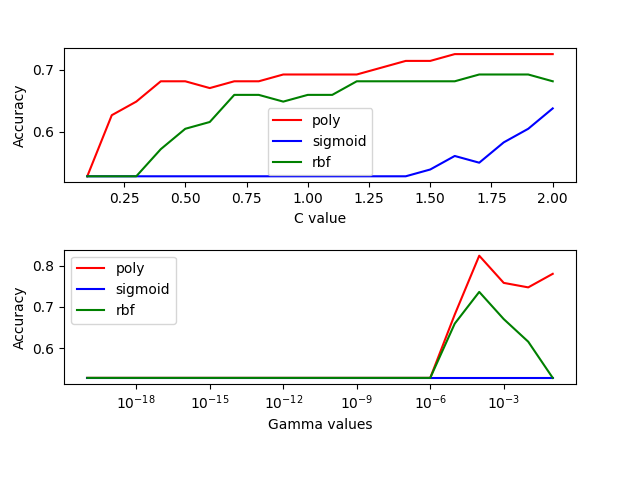
\includegraphics
                [width=0.8\textwidth,keepaspectratio]
                {img/svm_chart_heart.png}
                \caption
                [svm chart heart]{Wykres dokładności klasyfikacji, w zależności od
                wartości parametrów C i gamma, dla zbioru heart}
                \label{svm_chart_hearts}
            \end{figure}
            \FloatBarrier

%GESTURES

            \begin{table}[!htbp]
                \begin{minipage}{.35\textwidth}
                    \centering
                    \begin{tabular}{|c|c|}
                        \hline
                        C & Accuracy \\ \hline
                        0.1 & 0.3525 \\ \hline
                        0.2 & 0.403 \\ \hline
                        0.3 & 0.4389 \\ \hline
                        0.4 & 0.4655 \\ \hline
                        0.5 & 0.4951 \\ \hline
                        0.6 & 0.514 \\ \hline
                        0.7 & 0.5228 \\ \hline
                        0.8 & 0.5274 \\ \hline
                        0.9 & 0.5283 \\ \hline
                        1.0 & 0.528 \\ \hline
                        1.1 & 0.5265 \\ \hline
                        1.2 & 0.5283 \\ \hline
                        1.3 & 0.5297 \\ \hline
                        1.4 & 0.5317 \\ \hline
                        1.5 & 0.5305 \\ \hline
                        1.6 & 0.5317 \\ \hline
                        1.7 & 0.5305 \\ \hline
                        1.8 & 0.5303 \\ \hline
                        1.9 & 0.5308 \\ \hline
                        2.0 & 0.5317 \\ \hline
                    \end{tabular}
                    \caption
                    [svm table c gestures poly]{Zbiór gestures funkcja - wielomian}
                    \label{svm_table_c_gestures_poly}
                \end{minipage}
                \hfill
                \begin{minipage}{.3\textwidth}
                    \centering
                    \begin{tabular}{|c|c|}
                        \hline
                        C & Accuracy \\ \hline
                        0.1 & 0.718 \\ \hline
                        0.2 & 0.7811 \\ \hline
                        0.3 & 0.8074 \\ \hline
                        0.4 & 0.8251 \\ \hline
                        0.5 & 0.8353 \\ \hline
                        0.6 & 0.8479 \\ \hline
                        0.7 & 0.8522 \\ \hline
                        0.8 & 0.8602 \\ \hline
                        0.9 & 0.8653 \\ \hline
                        1.0 & 0.8687 \\ \hline
                        1.1 & 0.871 \\ \hline
                        1.2 & 0.8727 \\ \hline
                        1.3 & 0.8747 \\ \hline
                        1.4 & 0.8764 \\ \hline
                        1.5 & 0.8796 \\ \hline
                        1.6 & 0.8816 \\ \hline
                        1.7 & 0.8836 \\ \hline
                        1.8 & 0.8856 \\ \hline
                        1.9 & 0.8884 \\ \hline
                        2.0 & 0.8907 \\ \hline
                    \end{tabular}
                    \caption
                    [svm table c gestures rbf]{Zbiór gestures funkcja - RBF}
                    \label{{svm_table_c_gestures_rbf}}
                \end{minipage}
                \hfill
                \begin{minipage}{.3\textwidth}
                    \centering
                    \begin{tabular}{|c|c|}
                        \hline
                        C & Accuracy \\ \hline
                        0.1 & 0.2711 \\ \hline
                        0.2 & 0.2854 \\ \hline
                        0.3 & 0.276 \\ \hline
                        0.4 & 0.2603 \\ \hline
                        0.5 & 0.2489 \\ \hline
                        0.6 & 0.2403 \\ \hline
                        0.7 & 0.2357 \\ \hline
                        0.8 & 0.226 \\ \hline
                        0.9 & 0.216 \\ \hline
                        1.0 & 0.2135 \\ \hline
                        1.1 & 0.2126 \\ \hline
                        1.2 & 0.212 \\ \hline
                        1.3 & 0.2089 \\ \hline
                        1.4 & 0.2049 \\ \hline
                        1.5 & 0.2006 \\ \hline
                        1.6 & 0.1983 \\ \hline
                        1.7 & 0.1978 \\ \hline
                        1.8 & 0.1986 \\ \hline
                        1.9 & 0.1955 \\ \hline
                        2.0 & 0.1938 \\ \hline
                    \end{tabular}
                    \caption
                    [svm table c gestures sigmoid]{Zbiór gestures funkcja - Sigmoidalna}
                    \label{svm_table_c_gestures_sigmoid}
                \end{minipage}
            \end{table}
            \FloatBarrier
            \begin{table}[!htbp]
                \begin{minipage}{.35\textwidth}
                    \centering
                    \begin{tabular}{|c|c|}
                        \hline
                        Gamma & Accuracy \\ \hline
                        1e-20 & 0.2457 \\ \hline
                        1e-19 & 0.2457 \\ \hline
                        1e-18 & 0.2457 \\ \hline
                        1e-17 & 0.2457 \\ \hline
                        1e-16 & 0.2457 \\ \hline
                        1e-15 & 0.2457 \\ \hline
                        1e-14 & 0.2457 \\ \hline
                        1e-13 & 0.2457 \\ \hline
                        1e-12 & 0.2457 \\ \hline
                        1e-11 & 0.2457 \\ \hline
                        1e-10 & 0.2457 \\ \hline
                        1e-09 & 0.2457 \\ \hline
                        1e-08 & 0.2457 \\ \hline
                        1e-07 & 0.2457 \\ \hline
                        1e-06 & 0.2457 \\ \hline
                        1e-05 & 0.2623 \\ \hline
                        0.0001 & 0.5508 \\ \hline
                        0.001 & 0.5636 \\ \hline
                        0.01 & 0.5636 \\ \hline
                        0.1 & 0.5636 \\ \hline
                    \end{tabular}
                    \caption
                    [svm table gamma gestures poly]{Zbiór gestures funkcja - wielomian}
                    \label{svn_table_gamma_gestures_poly}
                \end{minipage}
                \hfill
                \begin{minipage}{.3\textwidth}
                    \centering
                    \begin{tabular}{|c|c|}
                        \hline
                        Gamma & Accuracy \\ \hline
                        1e-20 & 0.2457 \\ \hline
                        1e-19 & 0.2457 \\ \hline
                        1e-18 & 0.2457 \\ \hline
                        1e-17 & 0.2457 \\ \hline
                        1e-16 & 0.2457 \\ \hline
                        1e-15 & 0.2457 \\ \hline
                        1e-14 & 0.2457 \\ \hline
                        1e-13 & 0.2457 \\ \hline
                        1e-12 & 0.2457 \\ \hline
                        1e-11 & 0.2457 \\ \hline
                        1e-10 & 0.2457 \\ \hline
                        1e-09 & 0.2457 \\ \hline
                        1e-08 & 0.2457 \\ \hline
                        1e-07 & 0.2457 \\ \hline
                        1e-06 & 0.3159 \\ \hline
                        1e-05 & 0.6906 \\ \hline
                        0.0001 & 0.8821 \\ \hline
                        0.001 & 0.3459 \\ \hline
                        0.01 & 0.2457 \\ \hline
                        0.1 & 0.2457 \\ \hline
                    \end{tabular}
                    \caption
                    [svm table gamma gestures rbf]{Zbiór gestures funkcja - RBF}
                    \label{svn_table_gamma_gestures _rbf}
                \end{minipage}
                \hfill
                \begin{minipage}{.3\textwidth}
                    \centering
                    \begin{tabular}{|c|c|}
                        \hline
                        Gamma & Accuracy \\ \hline
                        1e-20 & 0.2457 \\ \hline
                        1e-19 & 0.2457 \\ \hline
                        1e-18 & 0.2457 \\ \hline
                        1e-17 & 0.2457 \\ \hline
                        1e-16 & 0.2457 \\ \hline
                        1e-15 & 0.2457 \\ \hline
                        1e-14 & 0.2457 \\ \hline
                        1e-13 & 0.2457 \\ \hline
                        1e-12 & 0.2457 \\ \hline
                        1e-11 & 0.2457 \\ \hline
                        1e-10 & 0.2457 \\ \hline
                        1e-09 & 0.2457 \\ \hline
                        1e-08 & 0.2457 \\ \hline
                        1e-07 & 0.2457 \\ \hline
                        1e-06 & 0.2594 \\ \hline
                        1e-05 & 0.3057 \\ \hline
                        0.0001 & 0.1655 \\ \hline
                        0.001 & 0.1515 \\ \hline
                        0.01 & 0.1513 \\ \hline
                        0.1 & 0.1424 \\ \hline
                    \end{tabular}
                    \caption
                    [svm table gamma gestures sigmoid]{Zbiór gestures funkcja - Sigmoidalna}
                    \label{svn_table_gamma_gestures_sigmoid}
                \end{minipage}
            \end{table}
            \FloatBarrier
            \begin{figure}[!htbp]
                \centering
                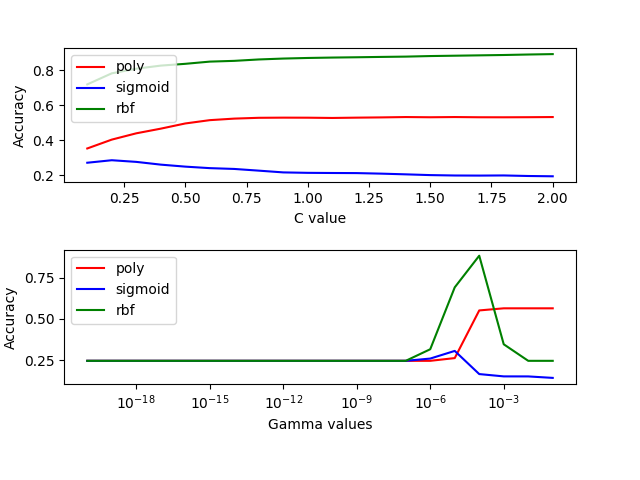
\includegraphics
                [width=0.8\textwidth,keepaspectratio]
                {img/svm_chart_gestures.png}
                \caption
                [svm chart gestures]{Wykres dokładności klasyfikacji, w zależności od wartości parametrów C i gamma, dla zbioru gestures}
                \label{svm_chart_gestures}
            \end{figure}
            \FloatBarrier

%WEATHER
            \begin{table}[!htbp]
                \begin{minipage}{.35\textwidth}
                    \centering
                    \begin{tabular}{|c|c|}
                        \hline
                        C & Accuracy \\ \hline
                        0.1 & 0.7781 \\ \hline
                        0.2 & 0.802 \\ \hline
                        0.3 & 0.8296 \\ \hline
                        0.4 & 0.8384 \\ \hline
                        0.5 & 0.842 \\ \hline
                        0.6 & 0.8443 \\ \hline
                        0.7 & 0.8446 \\ \hline
                        0.8 & 0.8458 \\ \hline
                        0.9 & 0.8461 \\ \hline
                        1.0 & 0.8468 \\ \hline
                        1.1 & 0.8476 \\ \hline
                        1.2 & 0.8477 \\ \hline
                        1.3 & 0.8484 \\ \hline
                        1.4 & 0.8485 \\ \hline
                        1.5 & 0.8486 \\ \hline
                        1.6 & 0.8488 \\ \hline
                        1.7 & 0.849 \\ \hline
                        1.8 & 0.8491 \\ \hline
                        1.9 & 0.8495 \\ \hline
                        2.0 & 0.8496 \\ \hline
                    \end{tabular}
                    \caption
                    [svm table c weather poly]{Zbiór weather funkcja - wielomian}
                    \label{svm_table_c_weather_poly}
                \end{minipage}
                \hfill
                \begin{minipage}{.3\textwidth}
                    \centering
                    \begin{tabular}{|c|c|}
                        \hline
                        C & Accuracy \\ \hline
                        0.1 & 0.7779 \\ \hline
                        0.2 & 0.778 \\ \hline
                        0.3 & 0.7807 \\ \hline
                        0.4 & 0.7921 \\ \hline
                        0.5 & 0.8101 \\ \hline
                        0.6 & 0.8219 \\ \hline
                        0.7 & 0.8306 \\ \hline
                        0.8 & 0.8361 \\ \hline
                        0.9 & 0.839 \\ \hline
                        1.0 & 0.8399 \\ \hline
                        1.1 & 0.8419 \\ \hline
                        1.2 & 0.8433 \\ \hline
                        1.3 & 0.8445 \\ \hline
                        1.4 & 0.8454 \\ \hline
                        1.5 & 0.8462 \\ \hline
                        1.6 & 0.8463 \\ \hline
                        1.7 & 0.8456 \\ \hline
                        1.8 & 0.8456 \\ \hline
                        1.9 & 0.8462 \\ \hline
                        2.0 & 0.8463 \\ \hline
                    \end{tabular}
                    \caption
                    [svm table c weather rbf]{Zbiór weather funkcja - RBF}
                    \label{svm_table_c_weather_rbf}
                \end{minipage}
                \hfill
                \begin{minipage}{.3\textwidth}
                    \centering
                    \begin{tabular}{|c|c|}
                        \hline
                        C & Accuracy \\ \hline
                        0.1 & 0.7779 \\ \hline
                        0.2 & 0.7779 \\ \hline
                        0.3 & 0.7779 \\ \hline
                        0.4 & 0.7779 \\ \hline
                        0.5 & 0.7779 \\ \hline
                        0.6 & 0.7779 \\ \hline
                        0.7 & 0.7779 \\ \hline
                        0.8 & 0.778 \\ \hline
                        0.9 & 0.778 \\ \hline
                        1.0 & 0.778 \\ \hline
                        1.1 & 0.778 \\ \hline
                        1.2 & 0.7781 \\ \hline
                        1.3 & 0.7785 \\ \hline
                        1.4 & 0.7792 \\ \hline
                        1.5 & 0.7799 \\ \hline
                        1.6 & 0.7807 \\ \hline
                        1.7 & 0.7821 \\ \hline
                        1.8 & 0.7834 \\ \hline
                        1.9 & 0.7848 \\ \hline
                        2.0 & 0.7862 \\ \hline
                    \end{tabular}
                    \caption
                    [svm table c weather sigmoid]{Zbiór weather funkcja - Sigmoidalna}
                    \label{svm_table_c_weather_sigmoid}
                \end{minipage}
            \end{table}
            \FloatBarrier
            \begin{table}[!htbp]
                \begin{minipage}{.35\textwidth}
                    \centering
                    \begin{tabular}{|c|c|}
                        \hline
                        Gamma & Accuracy \\ \hline
                        1e-21 & 0.7779 \\ \hline
                        1e-20 & 0.7779 \\ \hline
                        1e-19 & 0.7779 \\ \hline
                        1e-18 & 0.7779 \\ \hline
                        1e-17 & 0.7779 \\ \hline
                        1e-16 & 0.7779 \\ \hline
                        1e-15 & 0.7779 \\ \hline
                        1e-14 & 0.7779 \\ \hline
                        1e-13 & 0.7779 \\ \hline
                        1e-12 & 0.7779 \\ \hline
                        1e-11 & 0.7779 \\ \hline
                        1e-10 & 0.7779 \\ \hline
                        1e-09 & 0.7779 \\ \hline
                        1e-08 & 0.7779 \\ \hline
                        1e-07 & 0.7779 \\ \hline
                        1e-06 & 0.8515 \\ \hline
                        1e-05 & 0.8548 \\ \hline
                        0.0001 & 0.8559 \\ \hline
                        0.001 & 0.8561 \\ \hline
                        0.01 & 0.855 \\ \hline
                    \end{tabular}
                    \caption
                    [svm table gamma weather poly]{Zbiór weather funkcja - wielomian}
                    \label{svn_table_gamma_weather_poly}
                \end{minipage}
                \hfill
                \begin{minipage}{.3\textwidth}
                    \centering
                    \begin{tabular}{|c|c|}
                        \hline
                        Gamma & Accuracy \\ \hline
                        1e-21 & 0.7779 \\ \hline
                        1e-20 & 0.7779 \\ \hline
                        1e-19 & 0.7779 \\ \hline
                        1e-18 & 0.7779 \\ \hline
                        1e-17 & 0.7779 \\ \hline
                        1e-16 & 0.7779 \\ \hline
                        1e-15 & 0.7779 \\ \hline
                        1e-14 & 0.7779 \\ \hline
                        1e-13 & 0.7779 \\ \hline
                        1e-12 & 0.7779 \\ \hline
                        1e-11 & 0.7779 \\ \hline
                        1e-10 & 0.7779 \\ \hline
                        1e-09 & 0.7779 \\ \hline
                        1e-08 & 0.7779 \\ \hline
                        1e-07 & 0.778 \\ \hline
                        1e-06 & 0.8457 \\ \hline
                        1e-05 & 0.8526 \\ \hline
                        0.0001 & 0.8554 \\ \hline
                        0.001 & 0.8603 \\ \hline
                        0.01 & 0.7838 \\ \hline
                    \end{tabular}
                    \caption
                    [svm table gamma weather rbf]{Zbiór weather funkcja - RBF}
                    \label{svn_table_gamma_weather_rbf}
                \end{minipage}
                \hfill
                \begin{minipage}{.3\textwidth}
                    \centering
                    \begin{tabular}{|c|c|}
                        \hline
                        Gamma & Accuracy \\ \hline
                        1e-21 & 0.7779 \\ \hline
                        1e-20 & 0.7779 \\ \hline
                        1e-19 & 0.7779 \\ \hline
                        1e-18 & 0.7779 \\ \hline
                        1e-17 & 0.7779 \\ \hline
                        1e-16 & 0.7779 \\ \hline
                        1e-15 & 0.7779 \\ \hline
                        1e-14 & 0.7779 \\ \hline
                        1e-13 & 0.7779 \\ \hline
                        1e-12 & 0.7779 \\ \hline
                        1e-11 & 0.7779 \\ \hline
                        1e-10 & 0.7779 \\ \hline
                        1e-09 & 0.7779 \\ \hline
                        1e-08 & 0.7779 \\ \hline
                        1e-07 & 0.7779 \\ \hline
                        1e-06 & 0.7779 \\ \hline
                        1e-05 & 0.7779 \\ \hline
                        0.0001 & 0.7779 \\ \hline
                        0.001 & 0.7779 \\ \hline
                        0.01 & 0.7779 \\ \hline
                    \end{tabular}
                    \caption
                    [svm table gamma weather sigmoid]{Zbiór weather funkcja - Sigmoidalna}
                    \label{svn_table_gamma_weather_sigmoid}
                \end{minipage}
            \end{table}
            \FloatBarrier
            \begin{figure}[!htbp]
                \centering
                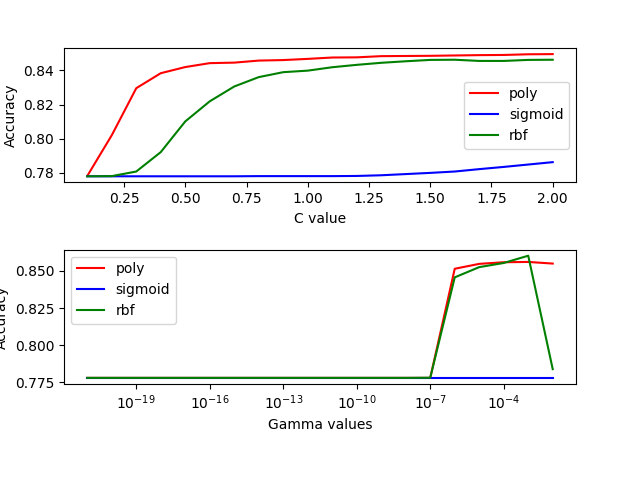
\includegraphics
                [width=0.8\textwidth,keepaspectratio]
                {img/svm_chart_weather.png}
                \caption
                [svm chart gestures]{Wykres dokładności klasyfikacji, w zależności od wartości parametrów C i gamma, dla zbioru weather}
                \label{svm_chart_weather}
            \end{figure}
            \FloatBarrier
        }

        \subsection{Drzewa decyzyjne i lasy losowe}
        \label{drzewa_decyzyjne_results} {
            \begin{figure}[h]
                \centering
                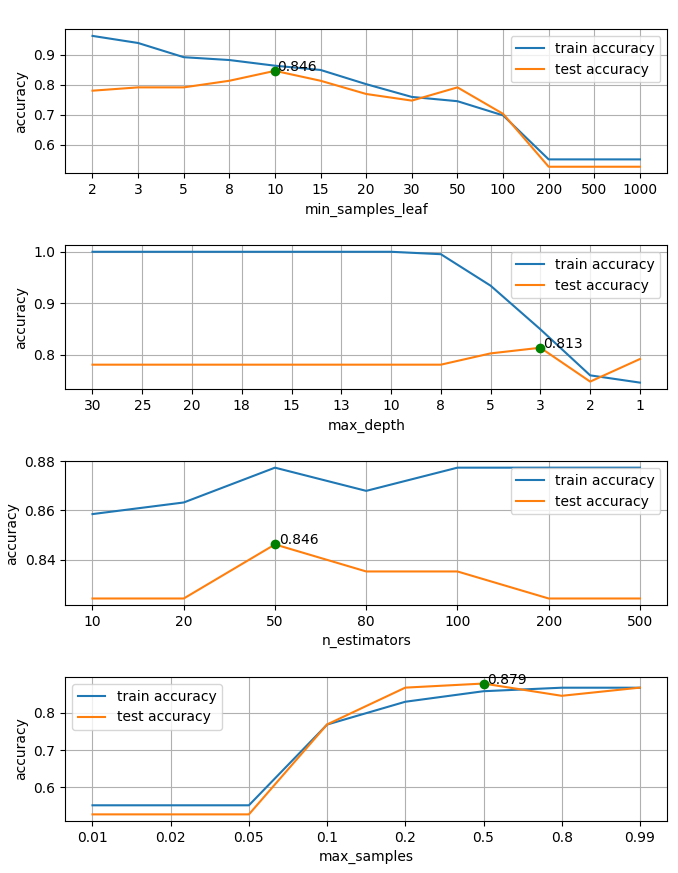
\includegraphics[width=0.96\textwidth]{img/mum_trees_1.png}
                \caption{Dokładność klasyfikacji drzewem decyzyjnym (dwa górne wykresy) i lasem losowym (dwa dolne wykresy) w zależności od parametrów dla zbioru \emph{heart disease}}
                \label{trees_hearts}
            \end{figure}
            \begin{figure}[h]
                \centering
                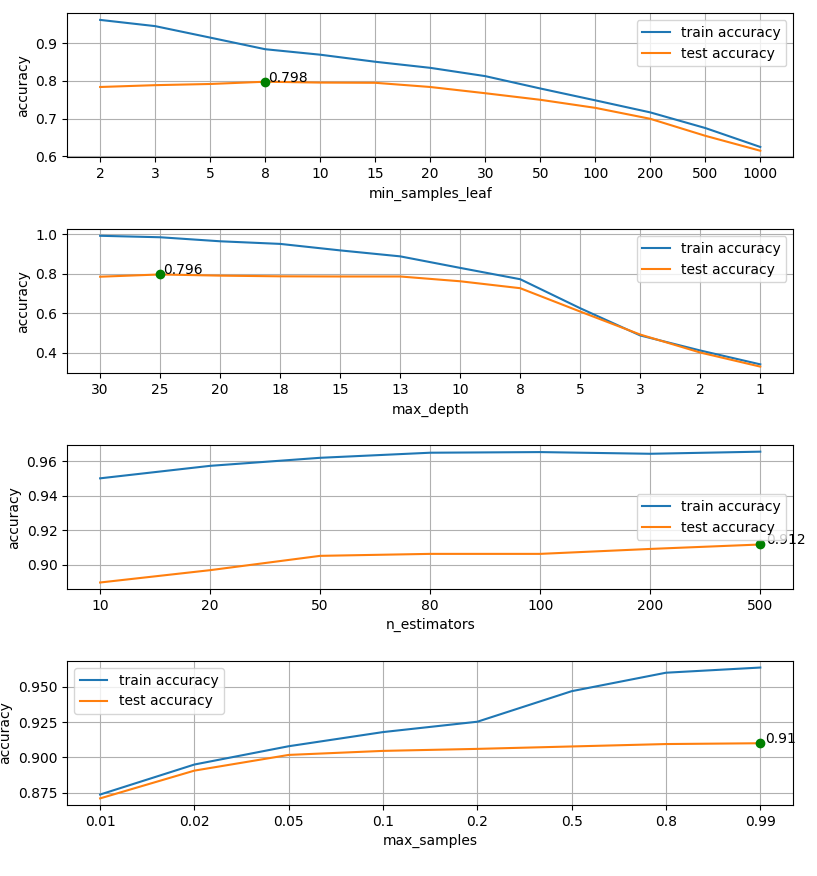
\includegraphics[width=\textwidth]{img/mum_trees_2.png}
                \caption{Dokładność klasyfikacji drzewem decyzyjnym (dwa górne wykresy) i lasem losowym (dwa dolne wykresy) w zależności od parametrów dla zbioru \emph{gestures}}
                \label{trees_gestures}
            \end{figure}
            \begin{figure}[h]
                \centering
                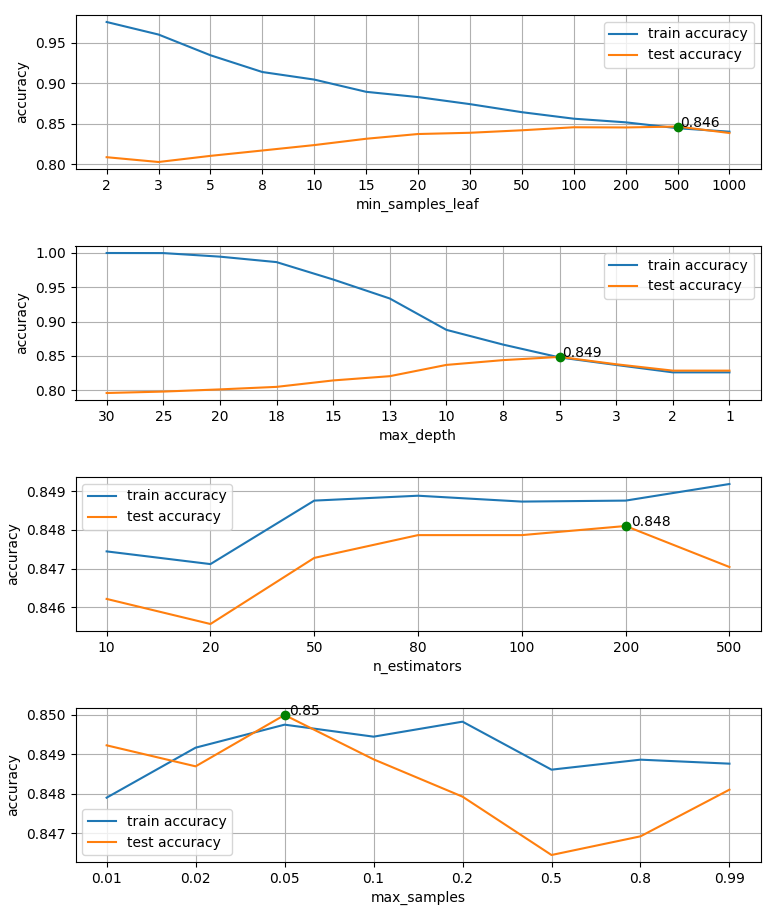
\includegraphics[width=\textwidth]{img/mum_trees_3.png}
                \caption{Dokładność klasyfikacji drzewem decyzyjnym (dwa górne wykresy) i lasem losowym (dwa dolne wykresy) w zależności od parametrów dla zbioru \emph{weather AUS}}
                \label{trees_weather}
            \end{figure}
            \FloatBarrier
        }
        
        \subsection{Porównanie klasyfikatorów}
        \label{porownanie} {
            \begin{table}[h]
                \begin{tabular}{|c|c|c|c|} \hline
                    Klasyfikator & Acc. \emph{hearts} & Acc. \emph{gestures} & Acc. \emph{weather} \\ \hline
                    K najbliższych sąsiadów & 0.736 & 0.683 & 0.854 \\
                    Naiwny klasyfikator Bayesa & 0.813 & 0.878 & 0.800 \\
                    Maszyna wektorów nośnych & 0.824 & 0.891 & 0.86 \\
                    Drzewa decyzyjne i lasy losowe & 0.879 & 0.912 & 0.85 \\ \hline
                \end{tabular}
                \caption{Porównanie najlepszych wyników klasyfikacji dla różnych algorytmów}
            \end{table}
            \FloatBarrier
        }
    }

    \section{Dyskusja}
    \label{summary} {

        \subsection{K-najbliższych sąsiadów}
        \label{knn_summary} {

            \subsubsection{Matryka Euklidesowa}
            \label{knn_summary_eucl} {

                W przypadku najmniejszego zbioru danych \textit{Heart disease}
                \cite{dataset_heart} dla wartości \textit{K=8} do \textit{K=11} można
                zauważyć znaczący wzrost wartości \textit{accuracy}. Co więcej
                dla \textit{K=10} udało się uzyskać najlepszy
                wynik. Wraz ze wzrostem parametru \textit{K} można zaobserwować delikatne
                unormowanie się wartości \textit{accuracy} - nie ma tak dużych różnich jak w przypadku
                mniejszych wartości parametru \textit{K}. Szczególną uwagę warto zwrócić na
                to, że dla wartości nieparzystych uzyskujemy znacząco lepsze wynik niż
                dla wartości parzystych. Stąd na wykresie można zobaczyć te `skoki`.
                Z literatury, sposobu działania tej metody zdrowej logiki jest to dosyć
                uzasadnione. W przypadku tego zbioru korzystanie z wartości parametru \textit{K} powyżej
                wartości 20 nie ma sensu gdyż wydłuża czas obliczeń a wyniki nie
                polepszają się.
                Biorąc pod uwagę zbiór \cite{dataset_heart} optymalnymi wartościami są te z
                przedziału od 7 do 11.

                W przypadku zbioru danych \textit{Gestures} \cite{dataset_gestures}, który
                jest zbiorem pośrednim jeżeli chodzi o jego wielkość to dla wartości
                \textit{K=3} oraz \textit{K=4} udało się uzyskać najlepszy wynik.
                Tak samo jak w przypadku zbioru \cite{dataset_heart} wartości parametru
                \textit{K} powyżej wartości 20 nie polepszają wyniku oraz wydłużają czas
                obliczeń. Warto zwrócić uwagę na fakt, że różnice między większością wartości
                parametru \textit{accuracy} jest w okolicach \textit{0.03} wiec wyniki dla
                wszystkich wartości parametru \textit{K} są praktycznie identyczne - są
                znacznie mniejsze odchylenia niż w przypadku zbioru \cite{dataset_heart}.
                Analizując wyniki i chcąc zoptymalizować dobór parametru \textit{K} autor
                sugeruje użycie wartości \textit{K} równej 3 do 7 z sugestią wyboru
                wartości nieprzystych.

                W przypadku ostatniego zbioru a jednocześnie największego o nazwie
                \textit{Weather AUS} \cite{dataset_weather_aus} najlepszy wynik udało się
                uzyskać dla wartości \textit{K=15}. Analogicznie jak w przypadku zbioru
                drugiego \cite{dataset_gestures} różnice pomiędzy uzyskanymi wynikami są
                bardzo niewielkie. Z ciekawych rzeczy, które można zauważyć jest to, że dla
                większych zbiorów danych aby uzyskać lepsze wyniki można pokusić sie o
                delikatne zwiększenie wartość parametru \textit{K} - zawsze warto to
                zweryfikować doświadczalnie. Sugerowane jest również korzystanie z
                wartości nieparzystych dla tego parametru.
            }

            \subsubsection{Matryka Manhattan}
            \label{knn_summary_manh} {

                W przypadku najmniejszego zbioru danych \textit{Heart disease}
                \cite{dataset_heart} dla wartości \textit{K=4} do \textit{K=7} można
                zauważyć znaczący wzrost wartości \textit{accuracy}. Co więcej
                dla \textit{K=4, K=5 K=7} udało się uzyskać najlepszy wynik. Wyniki i
                wnioski są dosyć zbliżone do tych w których została wykorzystana
                metryka Euklidesowa natomiast aby uzyskać zbliżone wyniki można było
                użyć mniejszej wartości parametru \textit{K}.

                W przypadku zbioru danych \textit{Gestures} \cite{dataset_gestures}, który
                jest zbiorem pośrednim jeżeli chodzi o jego wielkość to dla wartości
                \textit{K=5} udało się uzyskać najlepszy wynik. Analogicznie jak w
                przypadku metryki Euklidesowej różnice w wynikach są bardzo nieznaczne
                - autor domniemuje, że jest to kwestia charakterystyki zbioru danych.
                Zakres sugerowaych wartości parametru \textit{K} jest identyczny jak dla
                metryki Euklidesowej.

                W przypadku ostatniego zbioru a jednocześnie największego o nazwie
                \textit{Weather AUS} \cite{dataset_weather_aus} najlepszy wynik udało się
                uzyskać dla wartości \textit{K=17}. Analogicznie jak w dla metryki
                Euklidesowej różnice w wartościach \textit{accuracy} jest niezwykle
                mała natomiast była wymagana wieksza wartość parametru \textit{K} aby
                uzyskać maksimum wartości \textit{accuracy}. Również zalecane jest 
                korzystanie z wartości nieparzystych dla tego parametru - widać 
                ewidentne `skoki` na wykresie dla wartości nieprzystych.
            }
        }

        \subsection{Naiwny klasyfikator Bayesa}
        \label{bayes_summary} {
            Istnieje kilka wariantów naiwnego klasyfikatora Bayesa, które mogły zostać
            potencjalnie wykorzystane w zadaniu - \textit{wielomianowy},
            \textit{Bernoulliego} oraz \textit{Gaussa}.
            Wariant wielomianowy (\textit{ang. multinomial}) jest najczęściej
            wykorzystywany w przypadku analizy tekstu naturalnego i nie przyjmuje
            wartości ujemnych, a wariant \textit{Bernoulliego} sprawdza się dla
            wartości binarnych, dlatego zostały odrzucone podczas wykonywania zadania.
            Wariantem wykorzystanym podczas klasyfikacji był \textit{naiwny
            klasyfikator Gaussa}.

            Analizując otrzymane wyniki \textit{accuracy} można zauważyć, że są one
            zbliżone dla każdej wartości procent wykorzystanych danych jako zbiór
            testowy. Największe różnice można zauważyć w przypadku zbioru \textit{Heart
            disease} \cite{dataset_heart}, ale wynika to z jego małego rozmiaru.

            Nawet dla ekstremalnych wartości procent danych testowych jak 85\%, czy
            90\% klasyfikator osiągał wysokie wartości \textit{accuracy}. Kluczową
            kwestią wpływającą na wynik klasyfikacji był zatem sam dobór zbioru, jego
            liczebność oraz cechy.
        }

        \subsection{Maszyna wektorów nośnych}
        \label{svm_summary} {
            Dla zbioru \textit{Heart disease} \cite{dataset_heart} warto rozważyć
            wykorzystanie jako funkcji jądra - funkcji wielomianowej, dla której
            zanotowano najlepsze rezultaty klasyfikacji, zarówno dla parametru \emph{C}
            jak i \emph{Gamma}. Aby móc zarekomendować wykorzystanie funkcji
            sigmoidalnej należałoby kontynuować eksperymenty dla innych wartości
            parametrów. Na wykresie \ref{svm_chart_hearts}, możemy zauważyć tendencję
            wzrostową dokładności klasyfikacji dla wartości parametru \emph{C} z
            przedziału [1,7; 2,0], można zatem wnioskować że będzie się ona utrzymywać
            dla wartości wyższych i może uda się uzyskać wyższą dokładność klasyfikacji
            niż dla funkcji wielomianowej.

            Dla zbioru \textit{Gestures} \cite{dataset_gestures} rekomendowane jest
            wykorzystywanie funkcji RBF, manipulacja parametrem \emph{C} nie wpływa w
            sposób szczególny na dokładności klasyfikacji danych należących do tego
            zbioru. Natomiast można zaobserwować dynamiczną zmianę dokładności
            klasyfikacji w zależności od parametru \emph{Gamma}, którego optymalną
            (zbadaną) wartością dla funkcji RBF jest 0,0001, co skutkuje dokładnością
            działania klasyfikatora na poziomie 88\%.

            Dla zbioru \textit{Weather AUS} \cite{dataset_weather_aus} sytuacja jest
            najbardziej interesująca ze wszystkich badanych zbiorów. Jest to skutek
            tego, że przy odpowiednim dobraniu parametrów, można uzyskać zbliżoną
            dokładność klasyfikacji (w okolicach 79\%-86\%) dla dwóch różnych funkcji
            jądra - dla funkcji wielomianowej oraz RBF. Aby rekomendować wykorzystanie
            funkcji sigmoidalnej, wymagane byłoby kontynuowanie eksperymentów, tak aby
            określić wartość parametru \emph{C}, które za skutkuje wzrostem dokładności
            klasyfikacji. W przedziale [1,5; 2,0] można zaobserwować delikatny wzrost
            dokładności dla tej funkcji.
        }

        \subsection{Drzewa decyzyjne i lasy losowe}
        \label{drzewa_decyzyjne_summary} {
            Wykresy na rysunkach \ref{trees_hearts}, \ref{trees_gestures} oraz
            \ref{trees_weather} prezentują wyniki klasyfikacji dla pojedynczego drzewa
            decyzyjnego i lasu losowego. Każdy z rysunków jest związany z jednym z
            trzech zbiorów danych. Każdy zawiera również 4 wykresy.

            Pierwsze dwa są poświęcone pojedynczemu drzewu decyzyjnemu. Przebadana
            została dokładność klasyfikacji w zależności od dwóch parametrów:
            \emph{min\_samples\_leaf} (minimalna liczba próbek w liściu), oraz
            \emph{max\_depth} (maksymalna wysokość drzewa). Oba te parametry służą
            regularyzacji drzewa decyzyjnego, które samo z siebie ma silną tendencję do
            przeuczania. Zarówno \emph{min\_samples\_leaf} jak i \emph{max\_depth} mają
            bardzo podobne zadanie i wystarczy właściwie zastosować jeden z nich, aby
            algorytm budujący drzewo zatrzymał się wystarczająco wcześnie. Wyniki dla
            każdego zbioru danych pokazują tę samą tendencję -- na początku (małe
            wartości \emph{min\_samples\_leaf} i duże wartości \emph{max\_depth}) model
            jest silnie przetrenowany, czyli osiąga dokładność bliską 1 dla zbioru
            uczącego i znacznie mniejszą dla zbioru testowego. Wraz z modyfikacją
            wartości tych parametrów obie krzywe (dla zbioru uczącego i testowego)
            zbliżają się do siebie. W pewnym momencie, podczas tego zbliżania lub na
            samym jego końcu, dokładność klasyfikacji na zbiorze testowym osiąga swoje
            maksimum (zielona kropka) i później obie krzywe konsekwentnie już maleją.
            Zachowanie to jest zgodne z oczekiwaniami, według których jeżeli będziemy
            coraz bardziej ograniczać swobodę modelu to w końcu uniemożliwimy mu naukę
            i będzie niedouczony. Przy analizie krzywych z dwóch pierwszych wykresów na
            każdym rysunku, warto zwrócić uwagę, że są one tym bardziej gładkie im
            większy zbiór danych podlega analizie.

            Jeżeli chodzi o szczegółowe wyniki eksperymentów dotyczących pojedynczego
            drzewa decyzyjnego, to dla pierwszego zbioru (\emph{heart disease}) udało
            się osiągnąć dokładność $0.846$ lub $0.813$, w zależności od parametru.
            Ostatecznie za najlepszy, wykorzystany przy uczeniu całego lasu, uznany
            został \emph{min\_samples\_leaf} = 10. Bardzo podobnie ma się sytuacja w
            przypadku zbioru \emph{gestures}, gdzie ten sam parametr przyjmujący bliską
            wartość równą 8, pozwolił osiągnąć dokładność klasyfikacji $0.798$. W
            trzecim zbiorze wreszcie przewagę zdobyło ograniczeni głębokości drzewa i
            to właśnie ten parametr, przyjmując wartość 5, pozwolił uzyskać dokładność
            klasyfikacji $0.849$. Najprawdopodobniej wynika to z faktu, że zbiór ten
            jest znacznie (kilkadziesiąt i kilkaset) razy większy od poprzednich. Tak
            więc można mniej ograniczyć wysokość drzew pozostawiając im wciąż dużą
            swobodę przy rozbudowie. Z kolei widać tutaj również, że najlepsza wartość
            parametru \emph{min\_samples\_leaf}, również ze względu na rozmiar zbioru,
            jest dużo większa niż dla poprzednich zbiorów danych.

            Druga para wykresów na każdym z trzech rysunków jest poświęcona wynikom dla
            lasu losowego. Na podstawie wyników klasyfikacji pojedynczego drzewa
            wybrany została najlepszy parametr wraz z najlepszą wartością
            (\emph{max\_depth} lub \emph{min\_samples\_leaf}), który następnie był
            wykorzystany do regularyzacji wszystkich drzew w lesie. Tak więc jeden z
            parametrów lasu losowego, dotyczący charakterystyki samych drzew, wybrany
            został na podstawie eksperymentów dla pojedynczego drzewa. Jeżeli chodzi o
            parametry dotyczące samego zespołu klasyfikatorów to zbadane zostały dwa:
            \emph{n\_estimators} (liczba drzew w lesie), oraz \emph{max\_samples}
            (liczba losowych próbek ze zbioru uczącego wykorzystana do uczenia
            pojedynczego drzewa). Tym razem najpierw wybrana została najlepsza
            znaleziona wartość \emph{n\_estimators} a następnie wykorzystana przy
            szukaniu najlepszej wartości \emph{max\_samples}. W ten sposób ostatecznie
            dla każdego zbioru wybrany został najlepszy model, osiągający najwyższą
            dokładność klasyfikacji.

            Przyglądając się wykresom dotyczącym lasu losowego warto zwrócić uwagę, że
            w większości przypadków osiąga on lepsze wyniki niż pojedyncze drzewo. Jest
            to oczywiście zachowanie jak najbardziej oczekiwane. Dla pierwszego zbioru
            danych najlepszy okazał się las 50 drzew, gdzie każde uczy się na podstawie
            połowy zbioru uczącego. Pozwoliło to osiągnąć dokładność $0.879$. Jeszcze
            przed wybraniem dobrej wartości parametru \emph{max\_samples} las sprawował
            się lepiej niż pojedyncze drzewo. Ostatecznie jednak przewaga zespołu
            klasyfikatorów nad jednym dla tego zbioru to dokładność większa o zaledwie
            kilka setnych. Drugi zbiór (\emph{gestures}) najlepiej pokazał przewagę
            lasu losowego nad jednym drzewem decyzyjnym. Uzyskana dokładność
            klasyfikacji jest większa o ponad jedną dziesiątą. Co ciekawe, ograniczenie
            wartości parametru \emph{max\_samples} z 1 (domyślna wartości przy
            testowaniu samego \emph{n\_estimators}) do 0.99, spowodowało minimalny
            spadek dokładności. Jednakże to właśnie wyniki dla tego zbioru pokazuje, że
            zespół drzew może znacząco poprawić jakość klasyfikacji, która ostatecznie
            wyniosła $0.91$. Prawdopodobnie zbiór ten ma dużą wariancję, które jest
            znacząco redukowana przez wprowadzenie zespołu klasyfikatorów. Ostatni i
            największy zbiór danych również ostatecznie został lepiej zaklasyfikowany
            przez las losowy niż pojedyncze drzewo. Różnica ta jest jednak bardzo
            niewielka i uzyskana została dokładność $0.85$. Co ciekawe, w przypadku
            badania wartości parametru \emph{n\_estimators} dla tego zbioru, najlepsza
            dokładność klasyfikacji całego zespołu drzew okazała się mniejsza nż
            pojedynczego drzewa. W ogóle warto zwrócić uwagę, że dla ostatniego zbioru
            danych wszystkie wyniki są bardzo do siebie zbliżone. Jest to
            najprawdopodobniej spowodowane obciążeniem tego zbioru -- większość
            przykładów należy do jednej klasy. Niestety wykorzystana w prezentacji
            wyników miara \emph{accuracy} nie pokazuje tego w żaden sposób. Należy więc
            z dystansem podejść do oceny jakości klasyfikacji dla ostatniego zbioru,
            która jest raczej niemożliwa na podstawie tylko tej miary.
        }
    }

    \section{Wnioski}
    \label{conclusions} {
        Podsumowując wykonane zadanie wnioskujemy, że:
        \begin{itemize}
            \item Wartość parametru \textit{K} raczej powinna być nieparzysta ze względu
            na sposób działania tego klasyfikatora. Testując dobór parametru \textit{K}
            warto zwracać uwagę na różnice bezwzględne między wynikami. Często różnice te są
            bardzo niewielkie a korzystając z mniejszej wartości \textit{K}
            przyspieszamy obliczenia
            \item Dokładność klasyfikacji w zależności od wartości parametru \emph{C}
            nie zmienia się tak dynamicznie jak w zależności od wartości
            parametru \emph{Gamma}, na skutek czego łatwiej jest znaleźć
            odpowiednią wartość tego parametru. Dodatkowo zwiększenie wartości
            \emph{Gamma} znacząco wydłuża czas nauki maszyny wektorów nośnych.
            \item Lasy losowe zazwyczaj radzą sobie lepiej niż pojedyncze drzewa
            decyzyjne, różnica ta jest czasami jednak bardzo niewielka w stosunku
            do dodatkowego czasu obliczeń wymaganego przy uczeniu całego zespołu
            klasyfikatorów
            \item Kluczowym parametrem dla klasyfikatora Bayesa jest sam
            dobór zbioru danych i jego charakterystyka
        \end{itemize}
    }

    \begin{thebibliography}{0}
        \bibitem{dataset_heart}{https://www.kaggle.com/ronitf/heart-disease-uci}
        \bibitem{dataset_gestures}{https://www.kaggle.com/kyr7plus/emg-4}
        \bibitem{dataset_weather_aus}
        {https://www.kaggle.com/jsphyg/weather-dataset-rattle-package}
    \end{thebibliography}

\end{document}
